%%%%%%%%%%%%%%%%%%%%%%%%%%%%%%%%%%%%%%%%%%%%%%%%%%%%%%%%%%%%%%%%%%%%%%%%%%%%%%%%
% apend2.tex
%%%%%%%%%%%%%%%%%%%%%%%%%%%%%%%%%%%%%%%%%%%%%%%%%%%%%%%%%%%%%%%%%%%%%%%%%%%%%%%%

\chapter{Diagramas do levantamento de requisitos}
\label{apend:diagramas-levantamento-requisitos}

Este apêndice reúne os principais diagramas produzidos para apoiar o
levantamento de requisitos apresentado na
Seção~\ref{sec:metod:requisitos}. Os arquivos originais foram mantidos
em formato SVG para preservar qualidade e facilitar edição posterior.
Para tornar a consulta mais estável no PDF, os diagramas são exibidos
abaixo em versão rasterizada incorporada ao documento. Os arquivos-fonte
originais permanecem disponíveis no diretório \texttt{imagens/}.

\section{Diagrama de casos de uso}
\label{apend:diagramas-levantamento-requisitos:casos-uso}

Representa os atores identificados e as principais funcionalidades
associadas à automação pedagógica no sistema analisado.

\begin{center}
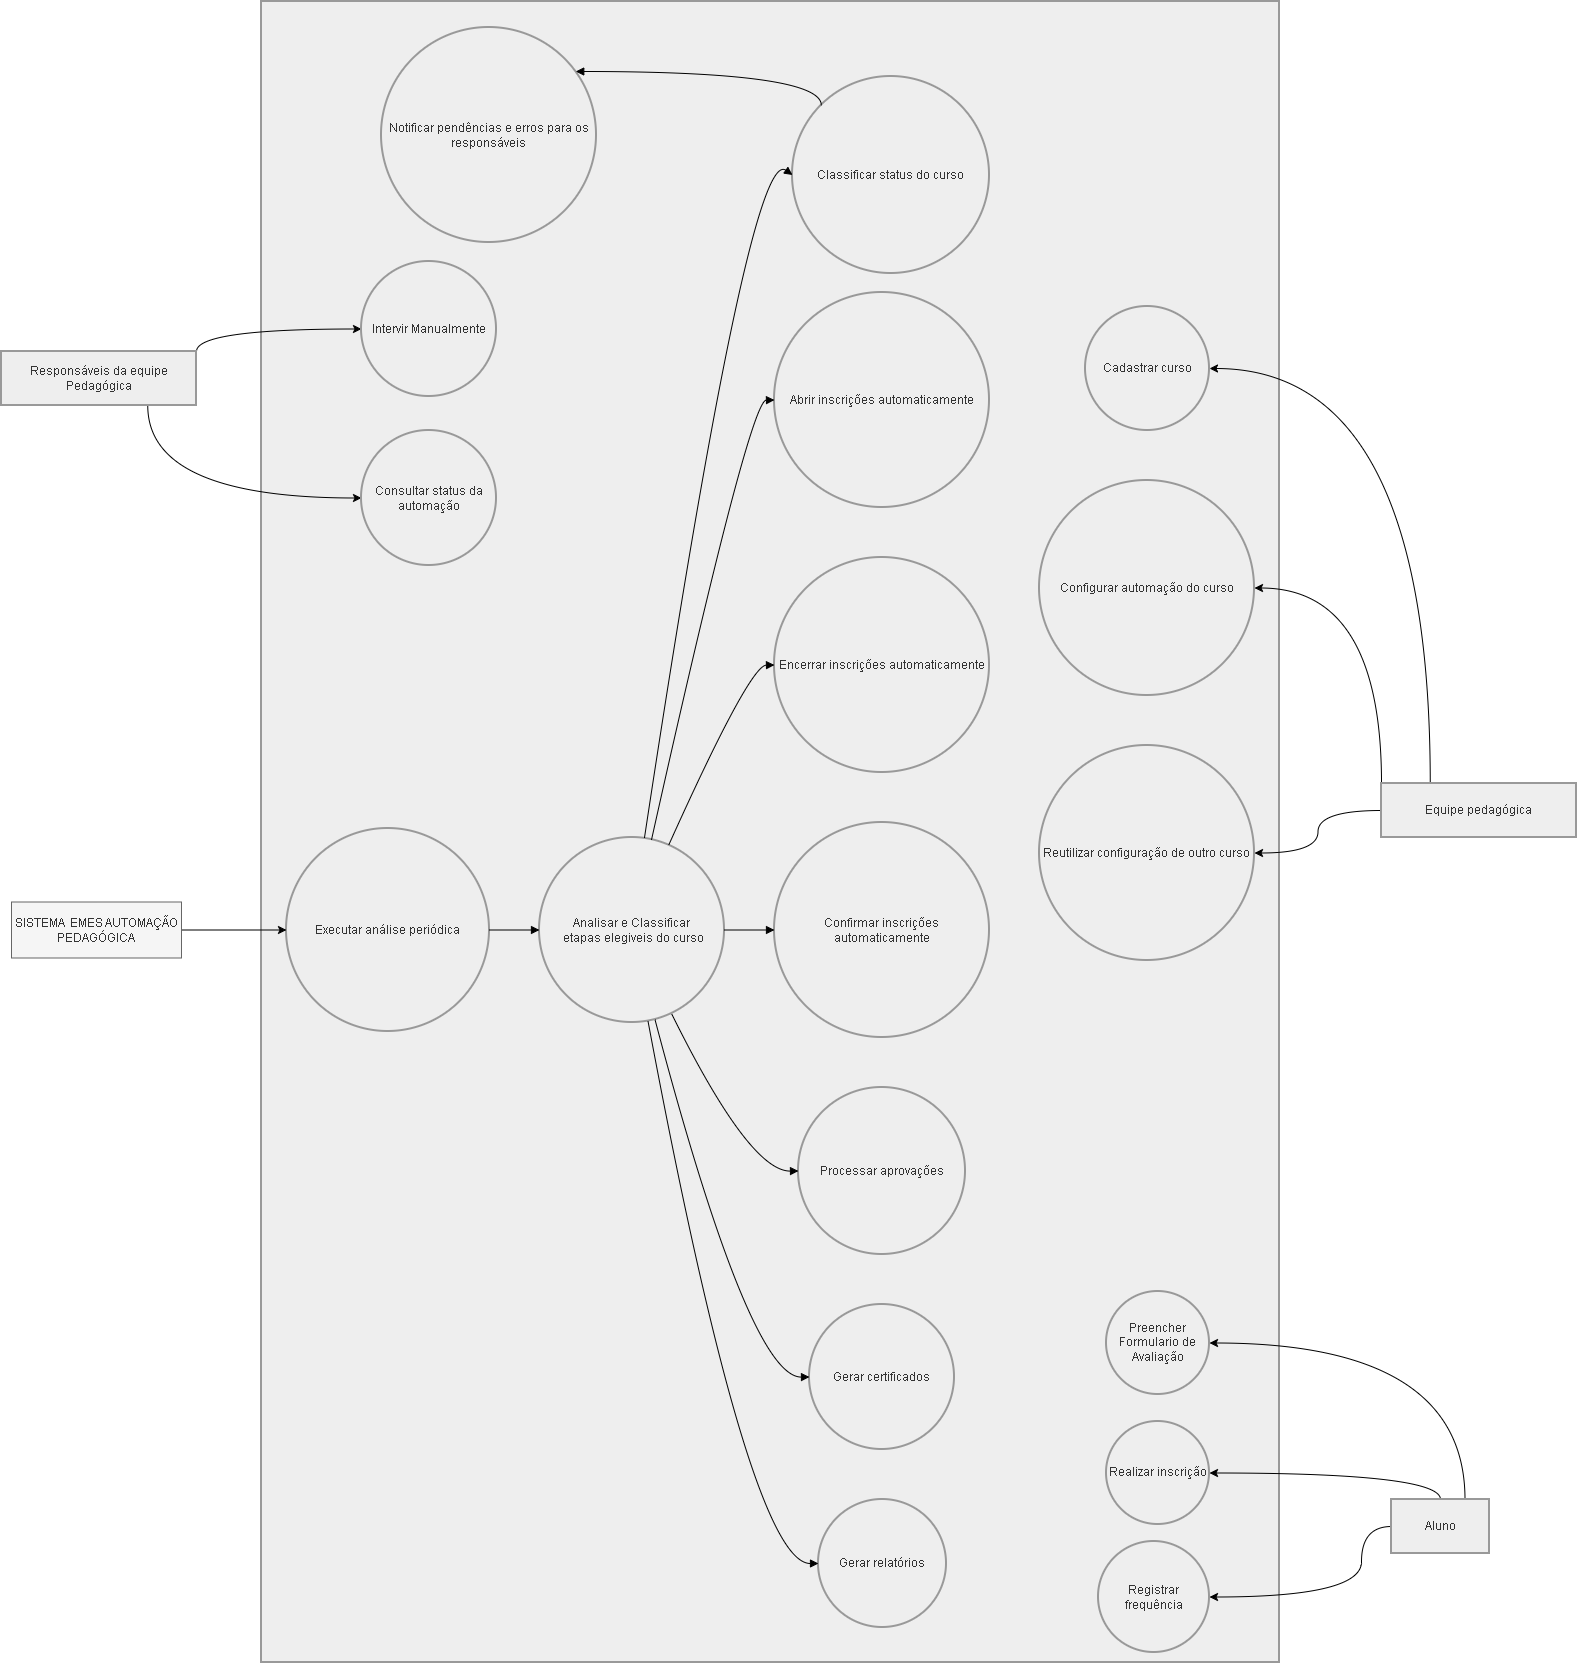
\includegraphics[width=\textwidth,height=0.82\textheight,keepaspectratio]{imagens/caso-de-uso.png}
\end{center}

% \noindent\textbf{Arquivo-fonte:} \texttt{imagens/caso-de-uso.svg}

\section{Diagrama de sequência}
\label{apend:diagramas-levantamento-requisitos:sequencia}

Apresenta, em nível abstrato, a sequência de interações esperadas entre
servidor pedagógico, sistema Educa EMES, sistema de automação e
responsável da equipe diante da execução automatizada ou do registro de
pendências.

\begin{center}
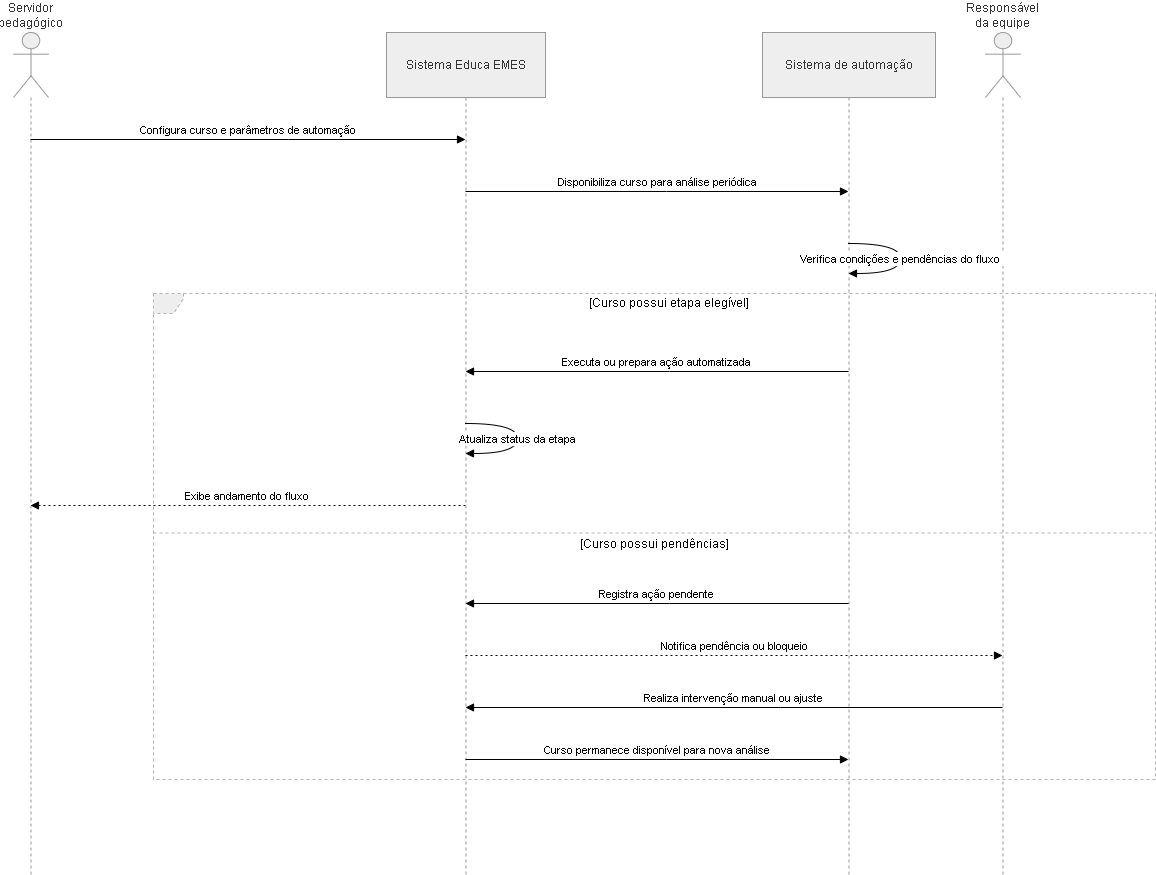
\includegraphics[width=\textwidth,height=0.72\textheight,keepaspectratio]{imagens/diagrama-sequencia-requisitos.png}
\end{center}

% \noindent\textbf{Arquivo-fonte:} \texttt{imagens/diagrama-sequencia-requisitos.svg}

\section{Fluxo geral da automação}
\label{apend:diagramas-levantamento-requisitos:fluxo-geral}

Resume o encadeamento macro da automação pedagógica, desde a
configuração do curso até a atualização de status e o tratamento de
pendências.

\begin{center}
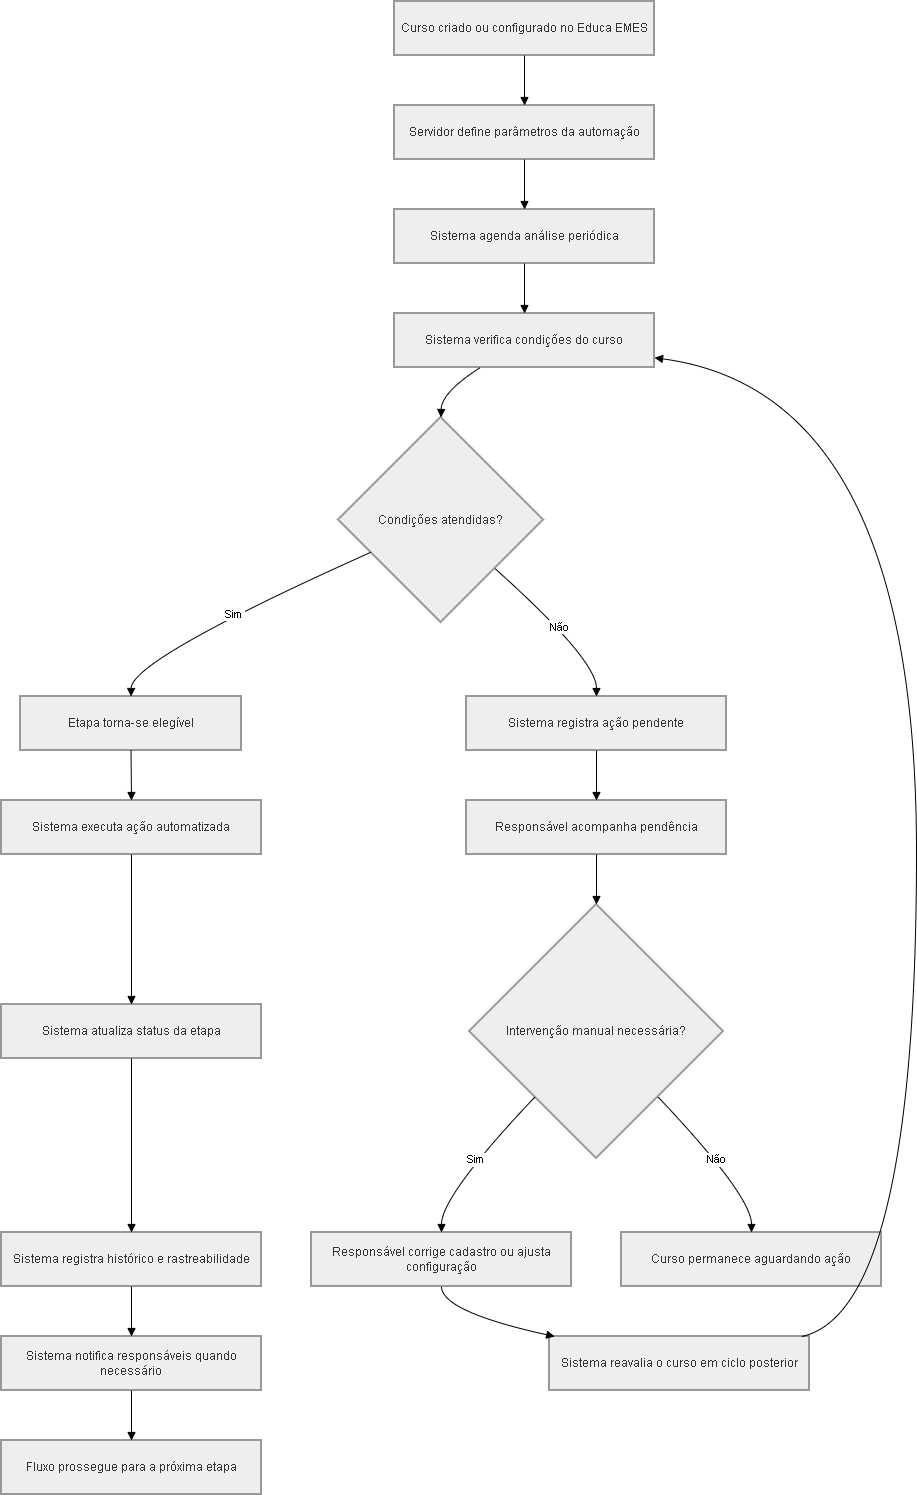
\includegraphics[width=\textwidth,height=0.82\textheight,keepaspectratio]{imagens/fluxo-automacao.png}
\end{center}

% \noindent\textbf{Arquivo-fonte:} \texttt{imagens/fluxo-automacao.svg}
